\section{Solution}\label{solution}

%2.5 pages
%Renan: Solucao-Intro
%Renan: Solucao-Manipulator
%Estevão: Solucao-Rails (Renan revision)
%Estevão/Renan: Solucao-Shutter
%TODO Gabriel: Solucao-Calibration

EMMA robotic technology is described in this section. The following system's
elements will be presented: the robotic manipulator; the customized modular
base; and the robot calibration. 

\begin{comment}
The Jirau's t urbine is the case study of
EMMA, thus a 3D CAD model was built with
SolidWorks\raisebox{1ex}{\textregistered} for simulation and solution analysis.

Its hardware is composed
of a mid-sized robotic manipulator, a customized modular rail base, and
vision-based sensors. As the manipulator cannot fully cover the blade's surface in a fixed
position, and the robot locomotion is complex in the turbine's environment, a
customized rail is designed to provide extra degrees of freedom (DOF) to the
system. EMMA aims to be a generic solution to large bulb type turbines, being
modular, and versatile. 
\end{comment}


\subsection{Robotic Manipulator}\label{manipulator}
The HVOF coating requirements and environment constraints demand a mid-sized
robotic manipulator (Sec.~\ref{hvof}). A survey was conducted to determine the
most adaptable off-the-shelf manipulator for the application. Overall simu\-lations and analysis were
performed using the OpenRave \cite{diankov2008openrave}, an environment for
simulating motion planning algorithms for robotics. There are several tools for
dynamics simulation of robots: Gazebo, V-Rep, Webots, and others%
% \cite{ivaldi2014tools}
. OpenRave was selected because of its integral design for real-time control
and execution monitoring, the core functionality for kinematics operations and
physics simulations, and the ROS support, simplifying future software
integration.

The simulations were performed to analyze the manipulator's work envelope in
the turbine, the required positions for full blade coating, the
manipulator's efforts (torque estimation), and to investigate possible
collisions with mechanical parts. The simulations steps are runner's
blade discretization, manipulator's base position computations for full cover,
and robotic manipulator's kinematics and dynamics.

The blade's surface discretization is an uniform sampling of the blade,
determining the manipulator's end-effector directions. The current approach
is to take the bounding box of the blade and sample its surface uniformly. Once the
surface of the box is sampled, the intersection of the blade and a ray
originating from each point going inward is taken. The normal of the blade's
surface from each of these intersection points is taken to be the end-effector
direction. %As an uniform sampling of the bounding box does not mean an uniform
%sampling of the blade, the box is oversampled, the blade's samples taken, and a
%k-d tree was generated to remove more than 10~mm close samples (filtering). 
The
resulting samples are translated 230~mm in respect with their normal vectors,
and collisions with the environment are checked.

Manipulator's base position computations are to uniformly sample the turbine's
confined space and to calculate the minimum required positions to process all
the blade's samples, considering angle and distance tolerances of the process.
It is a brute force search: for each position, inverse kinematics are computed
to determine the manipulator's joint parameters that provide the desired
positions and orientations of the end-effector.

The kinematic approach described above is not enough to ensure that the robot
will reach the samples. Maximum accelerations and torques should be investigated
and compared to the manipulator's specifications. To do this, we employ the
well know relation:
$\tau = M(q)\ddot{q} + C(q,\dot{q})\dot{q} + G(q)$
\cite{sciavicco2000differential}, where $\tau$ is the joints' torques, $M$ is
the matrix of moments of inertia estimated by manipulator's
CAD model, $q$ is the joints' angles, $C$ is the Coriolis matrix, and $G$ is the
gravity vector. The angular accelerations are derived by differential kinematics:
$\ddot{q}=J^\dagger(\ddot{x}-\dot{q}^TH\dot{q})$, where $H$ is the Hessian
matrix \cite{hourtash2005kinematic}, $\ddot{x}$ is the linear accelerations, and
$J^\dagger$ is the Jacobian matrix pseudoinverse. Therefore, torques can be
analytically estimated by the inverse dynamics in OpenRave.

% The typical path of HVOF coating is a zigzagging trajectory,
% i.e., it is a deceleration and acceleration process with direction changes. As
% the \textit{ex situ} solution uses a large-sized robotic manipulator, the
% end-effector's direction changes occur outside the blade's range, complying the
% speed requirement in the blade's range. However, while deceleration or
% acceleration, coating material is wasted to the environment or, most commonly,
% to a shadow plate.
% 
% The mid-sized robot for \textit{in situ} operation makes this strategy
% impossible, as, at some base positions, the robot will always be in the blade's
% range. The proposed solution modifies the original circuit of the gases that
% carry the coating particles to a new 2-way controlled circuit, in which there is
% a directional valve that changes the flow path from the thermal spray gun to return to tank
% circuit. The directional valve is autonomously actuated accordingly to the robotic
% manipulator's trajectory, i.e., the valve will ``shut'' while end-effector
% changes its direction. Therefore, the solution provides coating material
% savings, as the non-used particles are stored for future usage, and the hard
% coating speed requirement is met.

% \begin{figure}[h!]
%    \centering
%    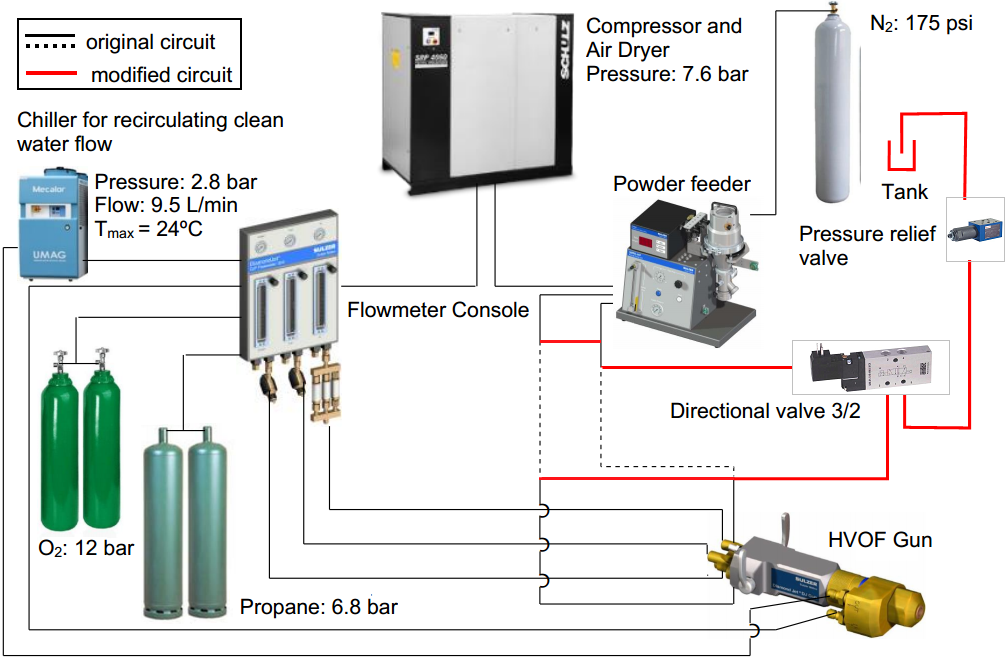
\includegraphics[width=0.9\columnwidth]{figs/mecanica/Circuito_HVOF_mod_en.PNG}
%    \caption{Simplified view of HVOF circuit with shutter}
%    \label{fig::circuito_hvof}
% \end{figure}

 

\subsection{Mechanical system}
% 0.75 pages

EMMA's mechanical system is non-actuated rails for manipulator's base
transportation, positioning and fixation. It comprises two rails, forming two
prismatic joints (P-P). The first rail is parallel to the
turbine axis, and it is responsible for the transportation of the manipulator from
hatch to close to the blade. The secondary rail is assembled from the first by
a rotational joint (R), which allows to position the upper rail parallel to the
blade's surface.

\begin{figure}
	\centering
	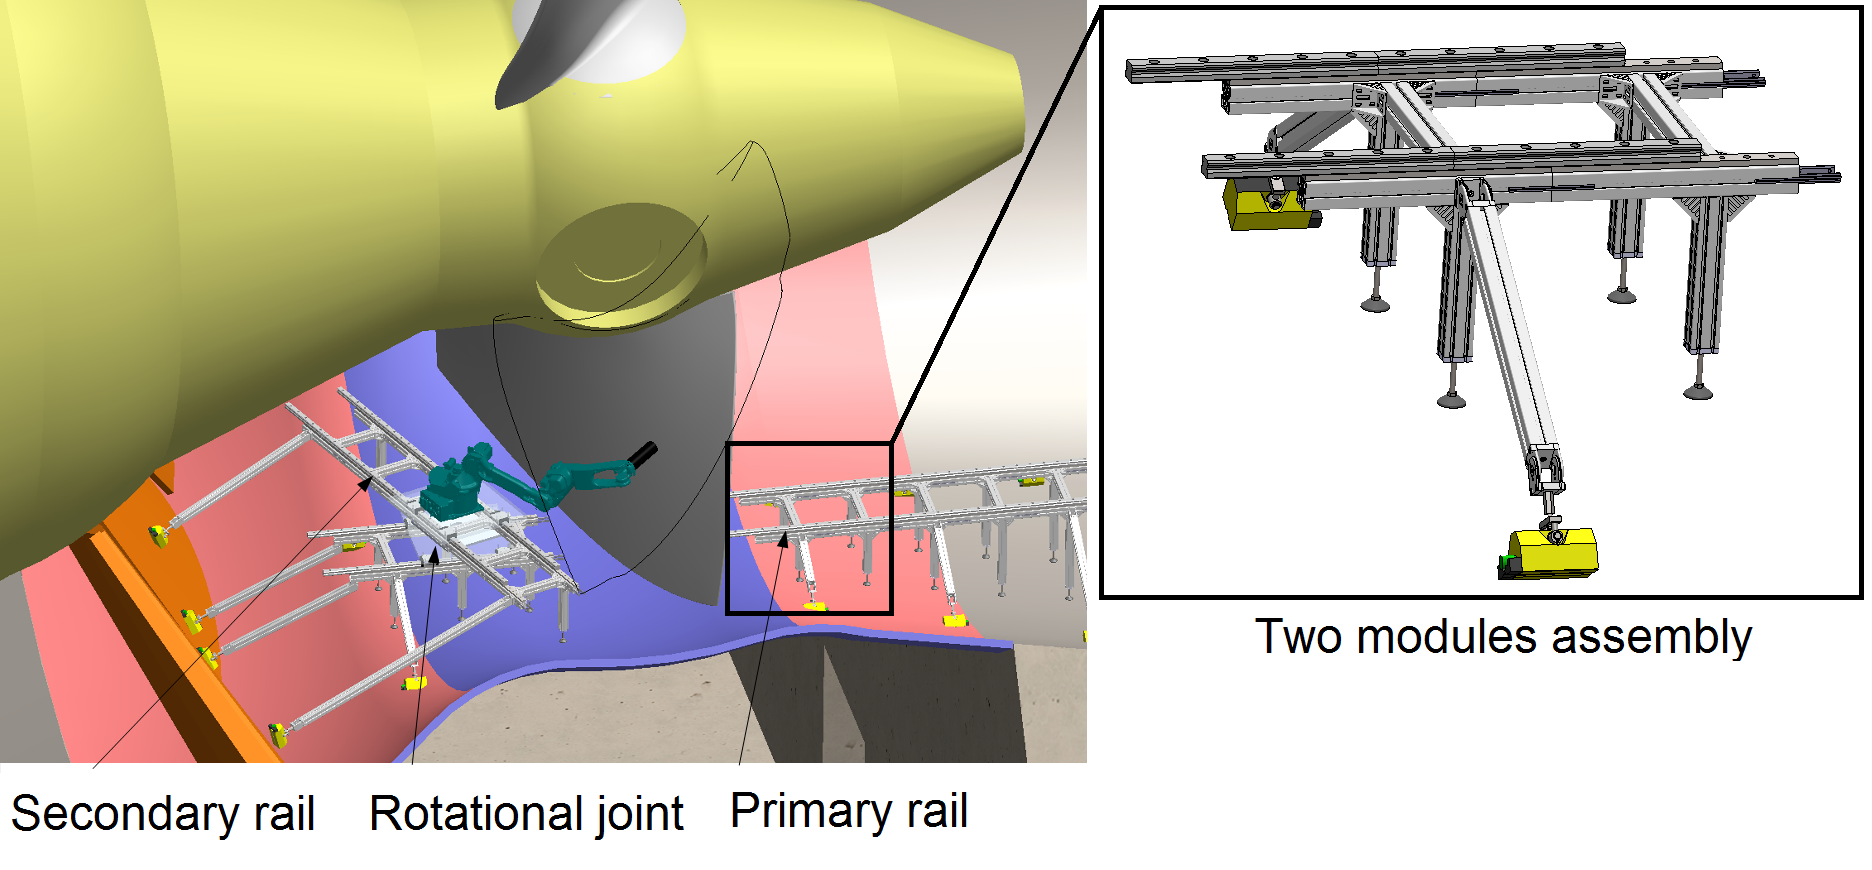
\includegraphics[width=1.0\columnwidth]{figs/mecanica/EMMA_Base_Secundaria_03.PNG}
    \caption{Customized base: primary and secondary rails.}
    \label{fig:base}
\end{figure}

The hatch limits the size of the rail in terms of weight
and geometry, thus a modular concept was adopted, such that the small modular
parts can be easily and manually assembled inside the turbine. Each module
contains all the necessary components to support, transport and position the
manipulator along it. Thus, the modules can be simply assembled in
sequence to increase the overall length of the prismatic joint.

A two parallel profiled rail system with a four carriage
setup\footnote{Profile Rail Guides LLT: Mounting maintenance and repair
instructions, SKF Group.} was adopted. %\cite{SKF_2013}.
This configuration creates a balanced force couple, eliminating the reaction
moments in each carriage. The frame structure is formed by aluminum
profile, since it is lightweight, corrosion resistant, geometrically flexible,
and modular (easy rail reconfiguration by changing few parts or adding anchor
arms).

The resulting frame structure is slender and lightweight, demanding careful
dynamic analysis of its integrity and stiffness. A Finite Element Analysis (FEA)
was performed to evaluate the stresses, strains and forces along the structure.
FEA is also used to specify the frame components, such as the profile's size,
and anchors quantity, dimensions, directions, and attachment points.

Since the draft tube and runner area are curved and sloped, properly fixing
the mechanical base is a major challenge in EMMA. The draft tube is composed of a
ferromagnetic steel material, hence magnetic fixtures is solution for
base attachment without environment modifications, as welding.

\begin{comment}
Common magnetic fixture products are temporary magnetic equipments used to hoist
and transport materials in an industrial plant. In EMMA, it is used to attach
and anchor the rail's modules to the ground.
\end{comment}

\subsection{Calibration}
 
The calibration process was divided in two different approaches depending on the
element to be localized and its caracteristics. The possibility to attach or
install markers in known positions dictated the strategies to be chosen,
therefore the calibration is separeted in the pose estimation of the robot and
of the blade, as follows.
   
The attachment of markers on the robotic manipulator can be performed with high
precision and repeatability, thus reflective spheres were chosen as reference
points in the process of robot localization. These spheres are identified inside
the point cloud by the 3D Hough Transform method \cite{camurri20143d}. The 3D
Hough Transform, as the 2D Hough Transform, is the search of an object on the
(discretized) parametric space. A sphere has four parameters: three for the
position of its center, and one for its radius. For each point on the point
cloud, it is assigned a collection of voxels on the discretized parametric
space, corresponding to the possible spheres passing through that point. As in a
voting process, the voxels with the greatest number of points assigned to define
the parameters of the most probable spheres. There might be computational issues
depending on the size of the parameter space, but it can be mitigated by
exploiting previous knowledge regarding the expected radius and viable region
for the robot inside the enviroment. Further improvements can be achieved
through the use of the normal vector at each point, exploiting the fact that
the center of the sphere is in the direction of the normal, thus reducing the
number of assigned voxels per point and in consequence the computational effort.

Fixing any marker on the blade would require its own calibration to ensure a
consistent reference point, thus the pose estimation of the blade must rely only
on the intrinsec properties of its surface geometry. The information must be extracted from
the point cloud (the scene) provided by the 3D laser sensor and
compared to a reference model previously stored. The characteristics of the point clouds are represented
by local descriptors, i.e., each interest point on the blade is associated
with a piece of information about its local neighborhood. Given the
sets of features from the model and the scence,  it is possible to determine the
correspondence between their descriptors. If enough correspondences are found
in the scene, above a threshold, the blade is identified and the position can be
determined \cite{Tombari2010a}.

As the blade is a large and smooth surface, the neighborhood of each point may
introduce similiar information, creating ambiguous descriptors that degrade the
matching perfomance, thus it is fundamental to wisely pick the interest points.
The ambiguous descriptors provide information about perpendicular translation to
the supporting plane, and the two rotations associated with it, thus no
information about the other DOFs, making the alignment to ``slide'' from the
correct transformation. Therefore, the interest points were sampled to
diversify the normal vectors' directions \cite{Rusinkiewicz2001}, allowing to
reduction of the number of samples to have a descriptor associated, when
compared to a uniform sampling, and maintaning the computational cost low.


Once the descriptors were estimated, the correspondences are determined if the
euclidean distance between a descriptor in the scene and in the model is lower
than a threshold. Each correspondence vote for a specific pose and scale factor in the
Hough space. After an instance of the model is found, it is performed the 
Iterative Closest Point (ICP) matching with the full resolution point clouds to
realize a fine alignment and compensate any discrepancy introduced by the
sampling. With the position of the blade and the manipulator in respect to a
common coordinate system, i.e., the origin of the laser sensor, it is possible
to determine the transformation between them and this information can be fed to
the trajectory and coverage algorithms. It is important to note that in every
step of the operation, in which either the manipulator base or the blade are
moved, there is the need to recalibrate the system.



